\documentclass{beamer}

% ----- Latex properties
\usepackage[latin1]{inputenc}
\usepackage{tikz} % 2D drawing
\usepackage{graphicx} % enhanced graphics
\graphicspath{ {img/} }

% ----- Beamer theme properties
\usetheme[left,hideothersubsections]{Goettingen}
\usecolortheme{crane,sidebartab}
\usefonttheme{structureitalicserif}
\useinnertheme[shadow]{rounded}

%\theoremstyle{definition}
\newtheorem{researchquestion}[theorem]{Research question}


% ----- Document properties
\title[Statistical Properties of DKD]
{%
\small
Investigating the Statistical Properties\\
of the Double Kernel Density Estimator\\
and its Applicability to a Multivariate Analysis\\
of Real World Health Data
}
\author[Harold Ship]
{%
Harold~Ship \\
    {%
    \small
    Advisors: Prof.~Boris~Portnov \and
    Dr.~Itai~Dattner \and
    Prof.~Em.~Benjamin~Reiser
    }
}
\institute[University~of~Haifa]
{%
University~of~Haifa \and 
Faculty~of~Management \and
Department~of~Information~\&~Knowledge~Management
}

\date{November 3, 2016}

% ----- The presentation
\begin{document}

% ----- Title page
\begin{frame}
\tikz [remember picture,overlay]
    \node at
        ([xshift=0.9cm, yshift=-3.6cm]current page.west) 
        {
\includegraphics[width=1.5cm]{univ_logo2.png}};
    \titlepage
\end{frame}

% ----- Table of Contents
\begin{frame}{Outline}
\tableofcontents
\end{frame}

% ----- SECTION: Theoretical Background
\section{Theoretical Background}

% ----- SUBSECTION: Measuring disease risk
\subsubsection{Measuring disease risk}

% ----- measuring disease risk slide
\begin{frame}\frametitle{Measuring disease risk}
    \begin{itemize}
        \item How do I measure the risk of developing a disease?
        \item How do I compare the problem of disease in different times and places?
    \end{itemize}
    \begin{definition}
        \alert{Cumulative incidence} or \alert{risk} is the proportion of the at-risk population that develop a disease during the study period.
        \begin{equation*}
            \lambda = \frac{number~of~new~cases~of~disease}{number~of~people~who~can~get~it}
        \end{equation*}
    \end{definition}
\end{frame}

% ----- SUBSECTION: Estimating disease risk with the double kernel density
\subsubsection{Estimating disease risk with the double kernel density}

\begin{frame}\frametitle{Smoothing disease cases}
    \begin{itemize}
        \item Are cases of disease concentrated in specific areas?
        \item Administrative boundaries: problematic
            \begin{itemize}
                \item Arbitrary boundaries
                \item Heterogenous populations
                \item Small number of cases: privacy
            \end{itemize}
        \item \alert{Kernel smoothing} to compute \emph{intensity} a.k.a \emph{density}
    \end{itemize}
    \begin{example}{\textbf{Left:} case locations. \textbf{Right:} intensity.}
    \centerline{
        \label{fig:points-and-dkd}
        \centering
        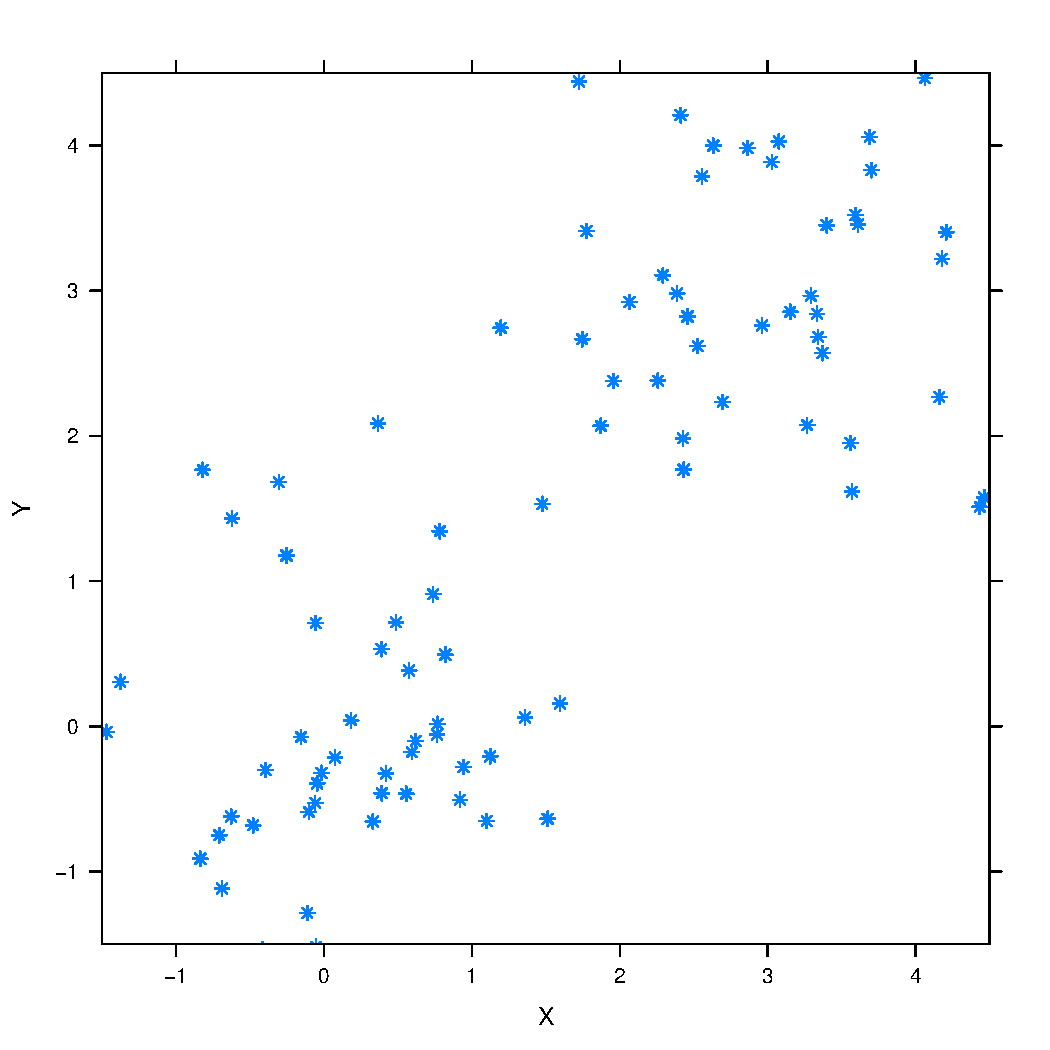
\includegraphics[width=0.4\textwidth]{example-incidents}
        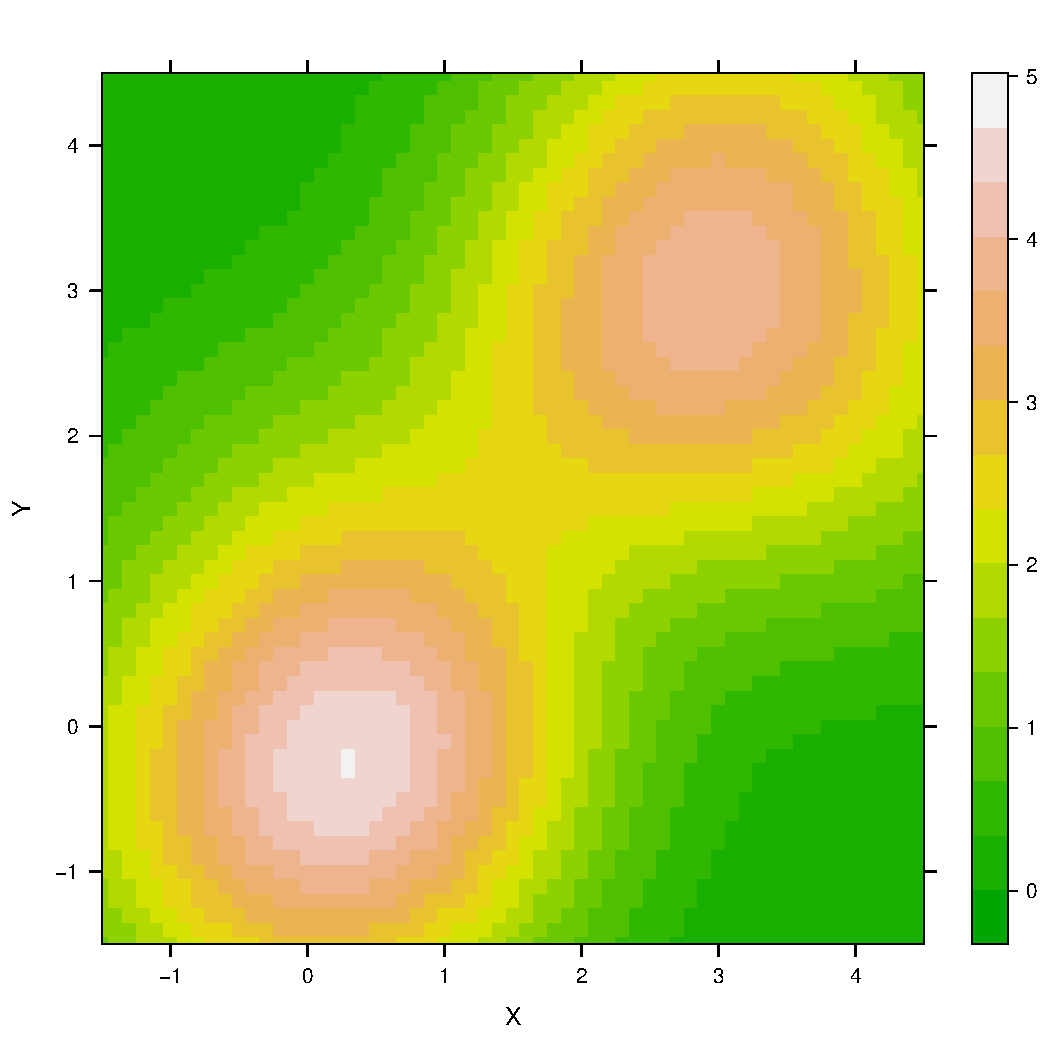
\includegraphics[width=0.4\textwidth]{example-incidents-smoothed}
        %\caption{About 100 simulated disease cases. \textbf{Left:} case locations. \textbf{Right:} intensity.}
    }
    \end{example}
\end{frame}

\begin{frame}\frametitle{Estimating disease risk with the double kernel density}
    \begin{itemize}
        \item Given: incident data
        \item Model: Poisson process
        \item Smooth: cases and population separately
        \item Divide: smoothed cases by smoothed population
        \item Result: double kernel density
    \end{itemize}
    \begin{definition}
        The \alert{double kernel density} is a function that is computed at a point by dividing the \emph{disease case intensity} by the \emph{population intensity} at that point.
        \begin{equation*}
            \hat{\lambda}_{dkd}(x,y) = \frac{ \hat{\lambda}_{c}(x,y) } { \hat{\lambda}_{p}(x,y) }
        \end{equation*}
    \end{definition}
\end{frame}

\begin{frame}\frametitle{Statistical thinking}
    \begin{itemize}
        \item Can we infer the \emph{risk} function from the data?
        \item If so, how good a job will the DKD do?
        \item Error functions: Mean squared error, mean absolute error, maximum error
        \item Peak location -- Euclidean distance, relative error of the height
        \item Expect estimated peak location to be correct, on average
        \item Expect estimated peak magnitude to be \alert{negative} since smoothing estimates towards average value
    \end{itemize}
\end{frame}


% ----- SECTION: Research Questions
\section{Research Questions}
\begin{frame}\frametitle{Research Questions}
    \begin{researchquestion}
        Under what conditions can the DKD be used to accurately estimate the true intensity function of a two-dimensional Poisson process, taking into account a variety of experimental setups?
    \end{researchquestion}
    \begin{researchquestion}
        How does the DKD perform in determining the magnitude and location of the peak of the intensity function of a two-dimensional Poisson process?
    \end{researchquestion}
\end{frame}

% ----- SECTION: Methodology
\section{Methodology}

% ----- SUBSECTION: Monte Carlo simulations
\subsubsection{Monte Carlo simulations of DKD}

\begin{frame}\frametitle{Monte Carlo simulations of DKD}
    \begin{itemize}
        \item Start with the ``truth''
        \item Simulation: generate a random sample of points
        \item Compare it to the ``truth''
        \item Repeat \textellipsis
    \end{itemize}
    \begin{itemize}
        \item Then see how the simulations are distributed
    \end{itemize}
\end{frame}

\begin{frame}\frametitle{How does bandwidth affect the error?}
    \begin{itemize}
        \item Too small -- high bias (undersmoothing)
        \item Too large -- high variance (oversmoothing)
    \end{itemize}
    \begin{example}{The best bandwidth is in \alert{red}.}
    \centerline{
        \label{fig:bandwidth-vs-error}
        \centering
        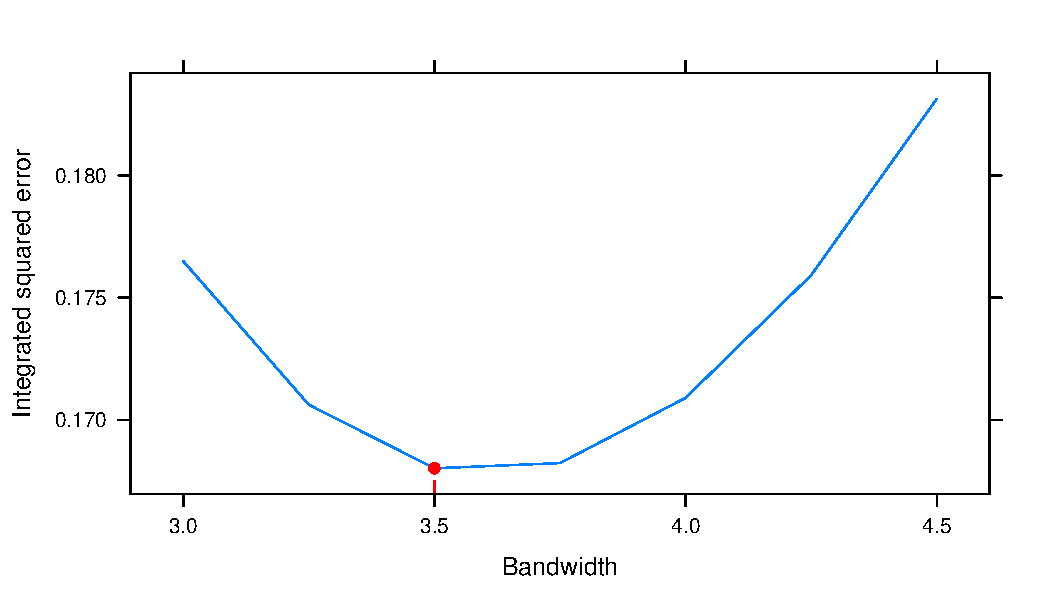
\includegraphics[width=0.9\textwidth]{error-bandwidth}
     }
    \end{example}
\end{frame}

\begin{frame}\frametitle{Evaluating the peaks}
    \begin{itemize}
        \item Single peak, centered at origin, moderate ``decay''
        \item Divide estimated peak value by ``true'' value
        \item Compute distance of estimated peak to ``true'' peak
    \end{itemize}
    \begin{example}
    \centerline{
        \label{fig:example-peaks}
        \centering
        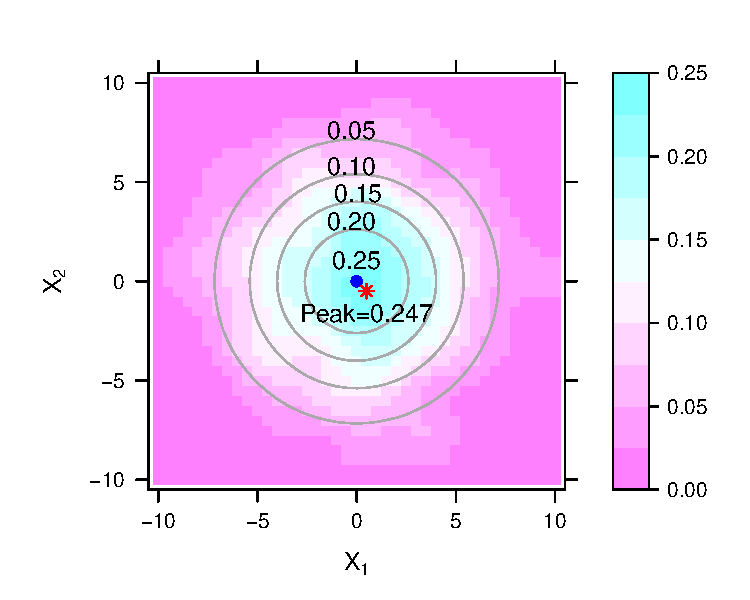
\includegraphics[width=0.8\textwidth]{example-peaks}
     }
    \end{example}
\end{frame}


% ----- SECTION: Results - Estimation Error
\section{Results}

% ----- SUBSECTION: Results of the DKD error
\subsubsection{Results of the DKD error analysis}
\begin{frame}\frametitle{Results of the DKD error analysis}
    \begin{itemize}
        \item TBD
    \end{itemize}
\end{frame}

% ----- SUBSECTION: Results of the magnitude and location of the peaks
\subsubsection{Results of the magnitude and location of the peaks}

\begin{frame}\frametitle{Results of the magnitude of the peaks}
    \begin{itemize}
        \item True value of the peak: 0.248
        \item Bias of peak value: -0.0224 (-9\%)
        \item Standard deviation: 0.0173. (7\%)
        \item 90\% had peak value \alert{less than} the truth
    \end{itemize}
    \begin{example}
    \centerline{
        \label{fig:peaks-values-hist}
        \centering
        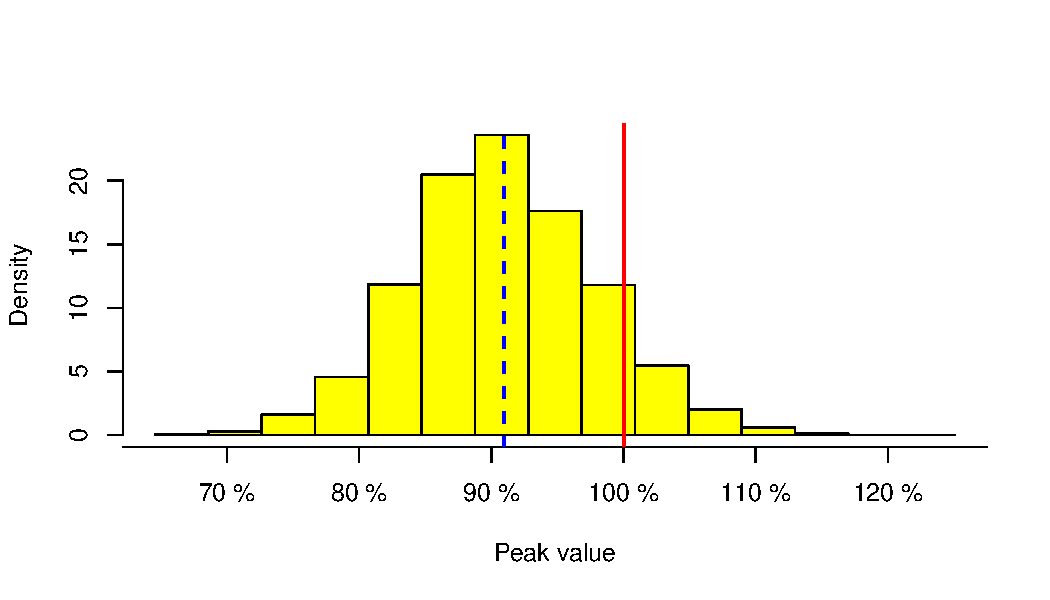
\includegraphics[width=0.9\textwidth]{peaks-hist-values}
     }
    \end{example}
\end{frame}

\begin{frame}\frametitle{Results of the location of the peaks}
    \begin{itemize}
        \item Average displacement of the peak: 0.833 (3.5\% of study area)
        \item Standard deviation:  0.466 (2\% of study area)
        \item 56\% of the simulations within 0.833 (4\%) of the truth
    \end{itemize}
    \begin{example}
    \centerline{
        \label{fig:peaks-loations-hist}
        \centering
        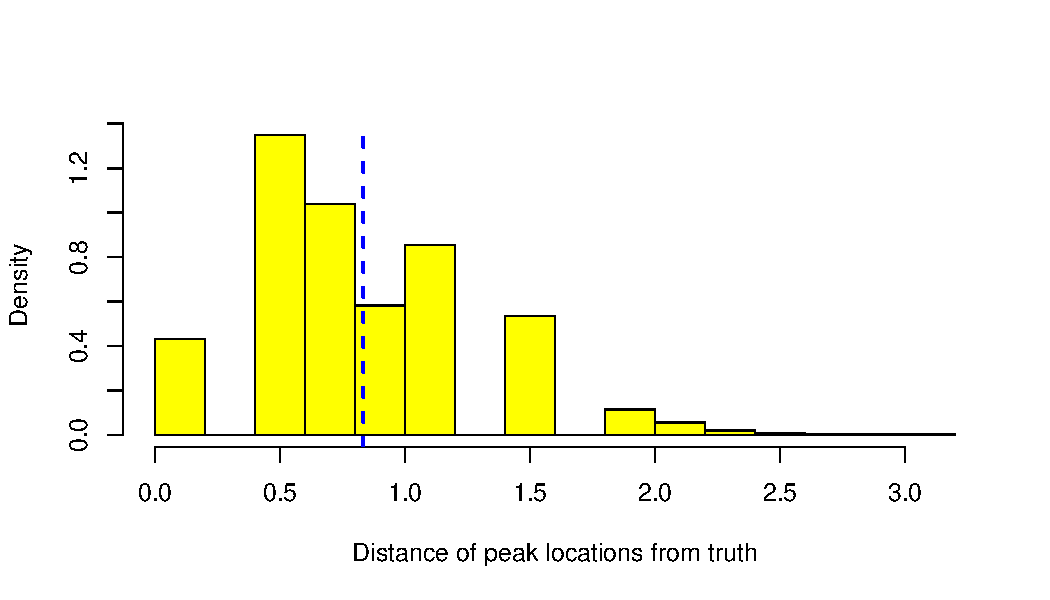
\includegraphics[width=0.9\textwidth]{peaks-hist-locations}
     }
    \end{example}
\end{frame}

% ----- SECTION: Discussion
\section{Discussion}

\begin{frame}\frametitle{Discussion}
    \begin{itemize}
        \item Calculated how well the DKD recovers a true intensity function by:
        \begin{itemize}
            \item Generating random samples from the ``truth'' using a simulated Poisson process
            \item Computing the DKD from the simulated data
        \end{itemize}
        \item Computed the empirical bias in the magnitude of the peak which is:
        \begin{itemize}
            \item Small (around 9\%)
            \item Negative, as expected
        \end{itemize}        
        \item Calculated the empirical bias in the location of the peak which is also small (within 3.5\%)
    \end{itemize}
\end{frame}

% ----- Next steps
\begin{frame}\frametitle{Next steps}
     For further research of this problem, we suggest the following:
     \begin{itemize}
         \item Vary the number of incidicents: use 200, 500, and 1,000
         \item Use different levels of ``concentration'' of the peak by varying the standard deviation of the ``truth'': 2, 4, 8
         \item Use a non-uniform population, one that also has a peak in the center of the study area
         \item Use cross-validation and Silverman's rule of thumb to calculate the bandwidth
         \item Compute the centroid of the top 5\% of the DKD values instead of the global maximum
     \end{itemize}
\end{frame}

% ----- SECTION: Learning Experience
\section{Learning Experience}
\begin{frame}\frametitle{Learning Experience}
\end{frame}

% ----- SECTION: Thank You
\section{Thank You}

\begin{frame}\frametitle{Thank You}
\end{frame}

\end{document}